\subsection{Lebegtetés}

%_
\begin{frame}
  A \emph{lebegtetés} egy speciális oldalelrendezési módszer, amivel egy elemet a tárolóján belül mozgathatunk.
  A \texttt{float} tulajdonsággal állítható a lebegtetés iránya:
  \begin{description}[m]
    \item[\texttt{left}] \hfill \\ A tároló bal széle felé mozdítja az elemet. Ha nincs ott elég hely, egy ,,sorral'' lejjebb helyezi el.
    \item[\texttt{right}] \hfill \\ Jobb oldalra mozgat.
    \item[\texttt{none}] \hfill \\ Nincs lebegtetés, alapértelmezés.
  \end{description}
  Legegyszerűbb és jellemző felhasználás: kép körbefolyatása szöveggel. Hibalehetőség: a lebegtetett elem túlnyúlhat a tárolón.
\end{frame}

%_
\begin{frame}
  \begin{columns}[c]
    \column{0.45\textwidth}
      \begin{exampleblock}{\textattachfile{lebeg1.html}{lebeg1.html}}
        \scriptsize
        \lstinputlisting[style=HTML,linerange={7-15},numbers=left,firstnumber=7]{lebeg1.html}
      \end{exampleblock}
    \column{0.45\textwidth}
      \begin{exampleblock}{}
        \scriptsize
        \lstinputlisting[style=HTML,linerange={16-28},numbers=right,firstnumber=16]{lebeg1.html}
      \end{exampleblock}
  \end{columns}
\end{frame}

%_
\begin{frame}
  \begin{columns}[c]
    \column{0.66\textwidth}
      \begin{exampleblock}{\textattachfile{lebeg1.html}{lebeg1.html}}
        \fontsize{7}{8} \selectfont
        \lstinputlisting[style=HTML,linerange={32-35},numbers=left,firstnumber=32]{lebeg1.html}
        \lstinputlisting[style=HTML,linerange={48-52},numbers=left,firstnumber=48]{lebeg1.html}
      \end{exampleblock}
    \column{0.3\textwidth}
      \begin{exampleblock}{}
        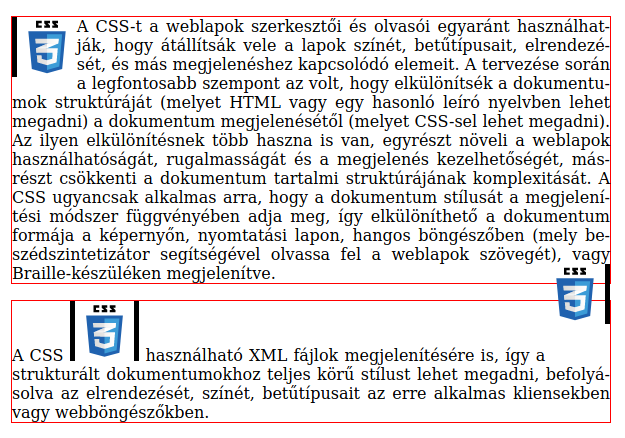
\includegraphics[width=\textwidth]{lebeg1.png}
      \end{exampleblock}
  \end{columns}
\end{frame}

%_
\begin{frame}
  Gyakran használják a lebegtetést az oldalelrendezés kialakítására, pl. tartalmak helytől függően egymás mellé vagy alá igazításához.
  \vfill
  \begin{center}
    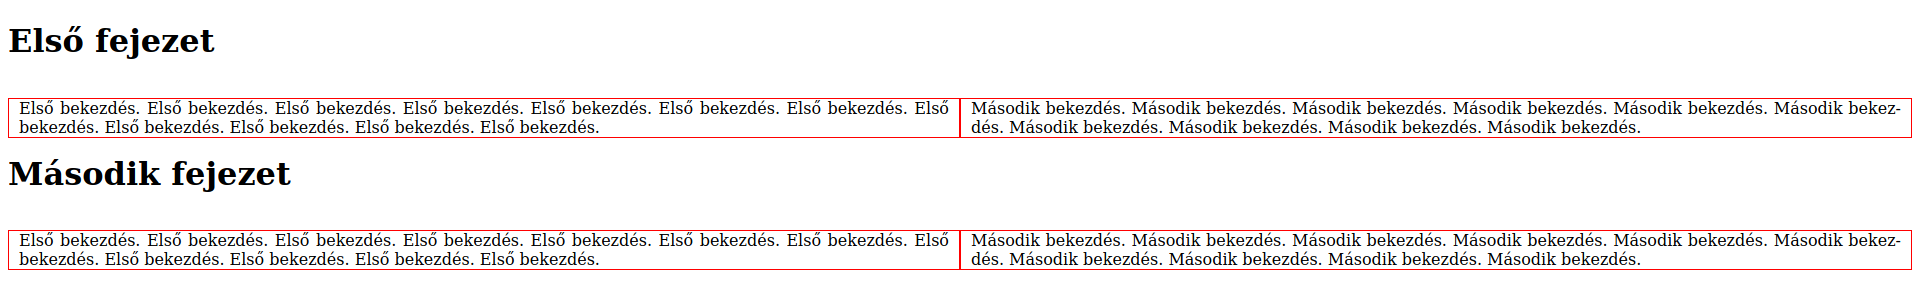
\includegraphics[width=\textwidth]{lebeg21.png}\\
    \textattachfile{lebeg2.html}{lebeg2.html}
  \end{center}
\end{frame}

%_
\begin{frame}
  \begin{columns}[c]
    \column{0.41\textwidth}
      \begin{exampleblock}{\textattachfile{lebeg2.html}{lebeg2.html}}
        \scriptsize
        \lstinputlisting[style=HTML,linerange={7-16},numbers=left,firstnumber=7]{lebeg2.html}
      \end{exampleblock}
    \column{0.54\textwidth}
      \begin{exampleblock}{}
        \scriptsize
        \lstinputlisting[style=HTML,linerange={20-28},numbers=right,firstnumber=20]{lebeg2.html}
      \end{exampleblock}
  \end{columns}
\end{frame}

%_
\begin{frame}
  Az oldalt lekicsinyítve viszont ismét kellemetlen mellékhatás lép fel:
  \vfill
  \begin{center}
    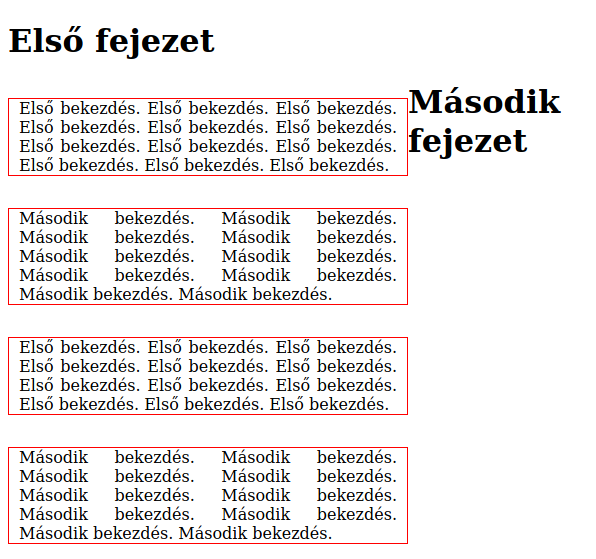
\includegraphics[width=.3\textwidth]{lebeg22.png}\\
    \textattachfile{lebeg2.html}{lebeg2.html}
  \end{center}
  Hogyan lehet úrrá lenni a gondokon?
\end{frame}

%_
\begin{frame}
  1. lehetőség: az \texttt{overflow} tulajdonság használata, de néha nem kívánt görgetősáv jelenik meg.
  \vfill
  \begin{columns}[c]
    \column{0.6\textwidth}
      \begin{exampleblock}{\textattachfile{lebeg3.html}{lebeg3.html}}
        \scriptsize
        \lstinputlisting[style=HTML,linerange={29-29},numbers=left,firstnumber=29]{lebeg3.html}
        \lstinputlisting[style=HTML,linerange={34-35},numbers=left,firstnumber=34]{lebeg3.html}
      \end{exampleblock}
    \column{0.35\textwidth}
      
\includegraphics[width=\textwidth]{lebeg3.png}
  \end{columns}
\end{frame}

%_
\begin{frame}
  \begin{columns}[c]
    \column{0.7\textwidth}
      \footnotesize
      2. lehetőség: a \texttt{clear} tulajdonsággal megadható, hogy egy elem valamely oldalán nem szerepelhet lebegtetett elem.
      \begin{description}[m]
        \item[\texttt{none}] \hfill \\ Az elem mindkét oldalára kerülhet lebegtetett másik elem, alapértelmezés.
        \item[\texttt{left}] \hfill \\ Az elem bal oldalára nem kerülhet lebegtetett elem.
        \item[\texttt{right}] \hfill \\ Ugyanaz a jobb oldalon.
        \item[\texttt{both}] \hfill \\ Egyik oldalon sem lehet lebegtetett elem.
      \end{description}
      \begin{exampleblock}{}
        \scriptsize
        \lstinputlisting[style=HTML,linerange={17-17},numbers=left,firstnumber=17]{lebeg4.html}
      \end{exampleblock}
    \column{0.25\textwidth}
      \begin{exampleblock}{\textattachfile{lebeg4.html}{lebeg4.html}}
        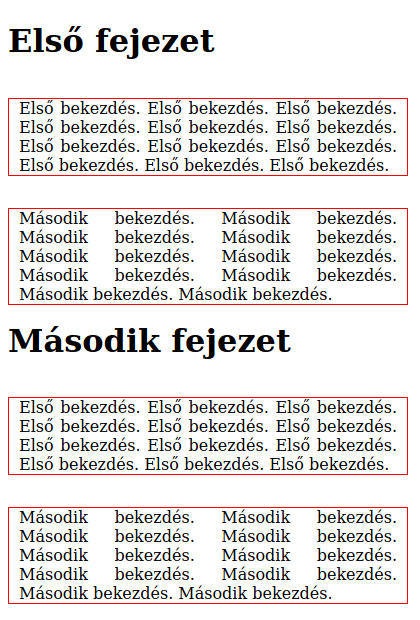
\includegraphics[width=\textwidth]{lebeg4.png}
      \end{exampleblock}
  \end{columns}
\end{frame}

%_
\begin{frame}
  \begin{columns}[c]
    \column{0.66\textwidth}
      3. lehetőség: a \emph{clearfix hack} (széles körben alkalmazott)
      \begin{exampleblock}{\textattachfile{lebeg5.html}{lebeg5.html}}
        \scriptsize
        \lstinputlisting[style=HTML,linerange={29-33},numbers=left,firstnumber=29]{lebeg5.html}
        \lstinputlisting[style=HTML,linerange={38-39},numbers=left,firstnumber=38]{lebeg5.html}
      \end{exampleblock}
    \column{0.3\textwidth}
      
\includegraphics[width=\textwidth]{lebeg5.png}
  \end{columns}
\end{frame}

%_
\begin{frame}
  \begin{columns}[T]
    \column{0.8\textwidth}
      \footnotesize
      Készítse el a Futókalandorok weboldalának \textattachfile{futokalandorok.html}{nyitóoldalát} az \hiv{\href{http://futokalandorok.hu/index.html}{eredeti oldal}} egyszerűsített változataként! (\textattachfile{futokalandorok.txt}{Nyers szöveg}.)
      \begin{itemize}
        \item Készítsen egy vízszintes elrendezésű menüt az oldal tetejére! Ha egy sorban nem férnek el a menüpontok, akkor azokat új sor(ok)ban kell elhelyezni.
        \item A menüsáv háttere halvány szürke.
        \item A ,,Futókalandorok'' főcím fekete, a menüpontok (most még sehová sem mutató) hivatkozásai középszürkék.
        \item Ha az egér a hivatkozás fölé kerül, színe feketére vált.
        \item A menü és a tartalmi rész között hagyjon ki egy kis helyet!
        \item A tartalmi rész két hasábos, melyek az oldal szélességének 50-50\%-át foglalják el. Hagyjon mindegyikben egy kis belső kitöltést!
        \item A bal hasábban jelenítse meg a \textattachfile{futokalandorok.svg}{logót}!
        \item A jobb hasáb utolsó bekezdését igazítsa jobbra!
      \end{itemize}
    \column{0.15\textwidth}
      
\includegraphics[width=\textwidth]{futokalandorok2.png}
  \end{columns}
\end{frame}

%_
\begin{frame}
  \begin{center}
    
\includegraphics[width=.75\textwidth]{futokalandorok1.png}\\
    \textattachfile{futokalandorok.html}{futokalandorok.html}
  \end{center}
\end{frame}
